% http://tex.stackexchange.com/questions/30720/footnote-without-a-marker
\newcommand\blfootnote[1]{%
  \begingroup
  \renewcommand\thefootnote{}\footnote{#1}%
  \addtocounter{footnote}{-1}%
  \endgroup
}

\part{Graphics and simulation hardware}
\frame{\partpage}

\begin{frame}{How computers work?}
		\textit{``A computer is like a small cardboard box. Inside this box lives an elf.
		The elf obeys instructions from my program, in the order they are given.
		Some instructions tell the elf to draw pictures onto the screen.''}
	\blfootnote{\url{https://blogs.msdn.microsoft.com/shawnhar/2008/03/31/an-elf-in-a-box/}}
\end{frame}

\begin{frame}{How computers really work}
		\textit{``A computer is like a cardboard box inhabited by a pair of elves,
		Charles Pitchwife Underhill plus his younger sibling George Pekkala Underhill 
		(both more commonly known by their initials).''}
	\blfootnote{\url{https://blogs.msdn.microsoft.com/shawnhar/2008/03/31/an-elf-in-a-box/}}
\end{frame}

\begin{frame}{How computers really work (cont.)}
		\textit{``Charles is smart, well educated, and fluent in dozens of languages 
		(C, C++, C\#, and Python, to name a few).
		George, on the other hand [...]
		finds it difficult to communicate with anyone other than his brother Charles, 
		prefers to plan his day well in advance, and gets flustered if asked to change 
		activities with insufficient warning. He has an amazing ability to multiply 
		floating point numbers, especially enjoying computations that involve vectors 
		and matrices.''}
	\blfootnote{\url{https://blogs.msdn.microsoft.com/shawnhar/2008/03/31/an-elf-in-a-box/}}
\end{frame}

\begin{frame}{How computers really work (cont.)}
		\textit{``When you run a program on this computer, Charles reads it and does whatever it says. 
		Any time he encounters a graphics drawing instruction, he notes that down on a piece of paper. 
		At some later point (when the paper fills up, or if he sees a Present instruction) 
		he translates the entire paper from the original language into a secret code which 
		only he and George can understand, then hands these translated instructions to his brother, 
		who carries them out.''}
	\blfootnote{\url{https://blogs.msdn.microsoft.com/shawnhar/2008/03/31/an-elf-in-a-box/}}
\end{frame}

\begin{frame}{CPUs vs GPUs}
	\begin{itemize}
		\pause \item (CPU = central processing unit; GPU = graphics processing unit)
		\pause \item GPUs are \textbf{highly parallelised}
			\begin{itemize}
				\pause \item Intel i7 6900K: \textbf{8} cores
				\pause \item Nvidia GTX 1080: \textbf{2560} shader processors
			\end{itemize}
		\pause \item GPUs are \textbf{highly specialised}
			\begin{itemize}
				\pause \item Optimised for floating-point calculations rather than logic
				\pause \item Optimised for performing the same calculation on several thousand vertices or pixels at once
			\end{itemize}
	\end{itemize}
\end{frame}

\begin{frame}{Physics processing unit}
	\begin{columns}
		\begin{column}{0.35\textwidth}
			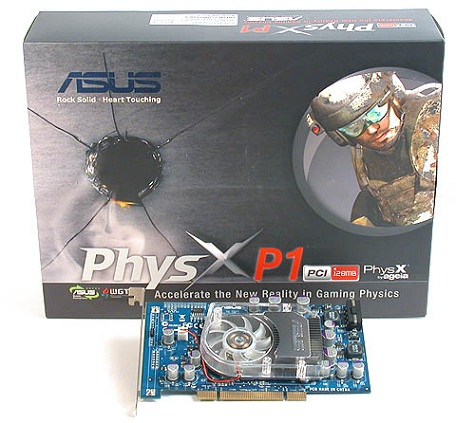
\includegraphics[width=\textwidth]{physx_ppu}
		\end{column}
		\begin{column}{0.63\textwidth}
			\begin{itemize}
				\pause \item Ageia PhysX PPU briefly appeared on the market in 2006-2008
				\pause \item Similar architecture to GPU (many cores, optimised for floating point calculations)
				\pause \item Ageia acquired in 2008 by Nvidia...
				\pause \item Now PhysX is Nvidia's middleware for performing physics simulation on the GPU
			\end{itemize}
		\end{column}
	\end{columns}
\end{frame}

\begin{frame}{General purpose GPU (GPGPU)}
	\begin{itemize}
		\pause \item Early GPUs used a \textbf{fixed pipeline} -- could only be used for rendering 3D graphics
		\pause \item Modern GPUs use a \textbf{programmable pipeline} -- can be programmed for other tasks
		\pause \item Physics simulation (e.g.\ PhysX)
		\pause \item Scientific computing (e.g.\ CUDA)
		\pause \item Deep learning
	\end{itemize}
\end{frame}

\begin{frame}{Graphics APIs}
	\begin{itemize}
		\pause\item Graphics APIs \textbf{abstract} away the differences between different manufacturers' GPUs
		\pause\item There are several APIs in use today:
		\begin{itemize}
			\pause\item \textbf{OpenGL}: Open standard, very mature, very widely supported
			\pause\item \textbf{Vulkan}: Open standard, very new, support still growing
			\pause\item \textbf{Direct3D}: Microsoft only
			\pause\item \textbf{Metal}: Apple only
			\pause\item Sony and Nintendo consoles have their own APIs; Microsoft consoles use Direct3D
		\end{itemize}
		\pause\item Most general-purpose game engines (e.g.\ Unity, Unreal) support several graphics APIs
		\pause\item On this module we will use \textbf{OpenGL} (but the principles are transferable)
	\end{itemize}
\end{frame}
